% 3 page
% \section{Potential Usage Under EDT}
% \label{sec:edt-debug-case}
% This section gives a concrete, minimal workflow showing how EDT enables
% \emph{distributed debugging} under a deterministic logical-time schedule. The key
% idea is to pause at a safe window boundary, inspect which nodes are scheduled
% next, and attach a native debugger to a specific client process (PID) while
% preserving reproducibility.

% \subsection{Start and pause at \(t=0\)}
% When running interactively, EDT prints a small command set and auto-pauses at
% \(t=0\) to provide a clean initial cut:

% \begin{verbatim}
% ** Commands: c | cN (e.g. c10) | n | p | s | s:<pid> | info | r | rN
% ** [auto-paused] t=0s
% \end{verbatim}

% \subsection{Inspect the next window and select a target process}
% \noindent\textbf{List next-window candidates.}
% At a pause point, the \texttt{s} command enumerates hosts scheduled in the next
% window, including each host's next-event time and the native PID(s) of its real
% client process(es). This provides an immediate mapping from \emph{logical time}
% to \emph{which real processes will execute next}.

% \begin{verbatim}
% s
% [next-window] t=...s window=[...--...]
%   host=geth-node          next_event=...   pid=3248123 (geth.1000)
%   host=prysm-beacon-1     next_event=...   pid=3248456 (beacon-chain.1000)
%   host=prysm-validator-1  next_event=...   pid=3248567 (validator.1000)
% \end{verbatim}

% \noindent\textbf{Optional: show more context.}
% The \texttt{info} command prints the boundary context (e.g., current time,
% window range, next global event), which is useful when aligning debugging with a
% suspected failing interval:

% \begin{verbatim}
% info
% [... paste your real terminal output here ...]
% \end{verbatim}

% \subsection{Attach a native debugger to one node}
% \noindent\textbf{Get an attach command.}
% Suppose we want to debug the geth node. We use \texttt{s:<pid>} to print a
% copy-pastable attach command:

% \begin{verbatim}
% s:3248123
% gdb -p 3248123
% \end{verbatim}

% \noindent\textbf{Why window boundaries enable ``distributed'' debugging.}
% EDT pauses at \emph{window boundaries} that correspond to the runahead-style safe
% horizon: within one window, hosts are guaranteed not to causally affect each
% other via cross-host deliveries. Therefore, the tester can focus on one target
% process (attach debugger, set breakpoints, single-step) while preserving a
% consistent global cut and a deterministic schedule for the rest of the system.

% \subsection{Step and continue deterministically}
% \noindent\textbf{Step one window.}
% The \texttt{n} command advances the system by exactly one window and pauses again
% at the next boundary. This is the natural ``next'' operation because the window
% is the minimal unit of safe parallel runahead:

% \begin{verbatim}
% n
% [... paste your real output here ...]
% \end{verbatim}

% \noindent\textbf{Continue until a target time.}
% To quickly reach a later region while keeping determinism, \texttt{cN} continues
% until logical time \(t=N\) seconds and then pauses:

% \begin{verbatim}
% c120
% [paused] t=120s
% \end{verbatim}

% \subsection{Lightweight replay via restart}
% When a failure is observed (or after enabling extra instrumentation), \texttt{rN}
% restarts from \(t=0\) and deterministically re-runs until \(t=N\) seconds,
% pausing at the same boundary:

% \begin{verbatim}
% r120
% ** restarting simulation in-process
% [paused] t=120s
% \end{verbatim}

% In practice, this workflow lets a tester reproduce and localize distributed
% failures by iterating on a single logical-time window: pause, inspect, attach,
% step, and replay, without relying on heavyweight snapshot mechanisms.



\section{Evaluation}
\label{sec:evaluation_methodology}

Our evaluation is designed to establish four properties of the time-decoupled testnet framework. First, it must be \emph{correct}: controlling logical time should preserve the key consensus behaviors expected from a real-time testnet, and executions should remain reproducible under fixed seeds and configurations. Second, it must be \emph{efficient}: decoupling protocol time from wall-clock time should reduce execution cost and improve scalability under a fixed machine budget. Third, it must be \emph{effective for testing}: by unlocking the time lock, it should substantially increase how densely the consensus state machine can be exercised under a fixed wall-clock budget. Fourth, it must be \emph{practical}: beyond accelerating execution, it should support new debugging and replay workflows that are difficult to realize on conventional real-time testnets.

Overall, our results show that the time-decoupled testnet (TDT) preserves key consensus behaviors, reproduces timing-sensitive executions under fixed seeds, delivers order-of-magnitude wall-clock speedups, increases core-logic execution density substantially enough to change the practical testing workflow for strongly time-controlled consensus, and enables replay/debugging-oriented operation on reproducible logical-time windows.

Concretely, our evaluation answers the following four questions:
\begin{itemize}
    \item \textbf{Q1} \emph{Fidelity and Reproducibility}: Does time-decoupled execution preserve key consensus behaviors, and can it reproduce the same timing-sensitive executions under fixed seeds and configurations?
    \item \textbf{Q2} \emph{Efficiency and Scalability}: How much wall-clock time does the time-decoupled testnet save, and how scalable is it compared to a real-time testnet?
    \item \textbf{Q3} \emph{Testing Effectiveness}: Under a fixed wall-clock testing budget, how much more of the consensus state machine can we exercise?
    \item \textbf{Q4} \emph{Operational Utility}: Can the framework support a practical replay-and-debug workflow for timing-sensitive consensus events, rather than merely accelerating execution?
\end{itemize}

\subsection{Experimental Setup}
\label{subsec:eval_setup}

Ethereum, as a widely used strongly time-controlled consensus protocol, is a natural testbed for our time-decoupled testnet framework. We focus on an Ethereum PoS testnet built from Prysm (v5.1.12) (with executable binaries \texttt{beacon-chain} and \texttt{validator}) and Geth.

We compare the time-decoupled testnet (TDT) with a real-time testnet (RT). Across RT and TDT, we keep client versions, launch command lines, and genesis states identical. The key difference is the execution model: RT binds protocol progress to wall-clock time over a local loopback deployment, whereas TDT virtualizes protocol time and executes over the DVN event-driven network model.
We emphasize that TDT does \emph{not} modify any protocol parameters (e.g., slot duration); it changes only how protocol time is realized during execution, while preserving protocol-time semantics. Unless otherwise stated, TDT experiments use fixed seeds so that the same timing-sensitive execution can be reproduced across repeated runs. The exact network size, peer topology, and evaluation window vary by question and are specified in the corresponding subsections.
All experiments run on Windows Subsystem for Linux (WSL) on Windows 11 with an AMD Ryzen 9 9950X CPU (16 cores and 32 threads) and 32\,GB RAM allocated to WSL.


\subsection{Fidelity and Reproducibility}
\label{subsec:eval_fidelity}

\begin{table*}[t]
\centering
\caption{Fidelity comparison between the time-decoupled testnet (TDT) and the real-time testnet (RT) (4 beacon nodes, 16 validators; evaluated slot range 16--271). Growth measures per-node block synchronization (256/256 slots). Reorg counts reflect observed chain-reorg warnings; TDT reorgs are shallow under the intentionally noisy latency model used for the reproducibility discussion. Finality tracks finalized epoch progression. Attestations are derived from validator ``previous epoch aggregated voting summary'' over epochs 1--7, excluding the startup epoch.}
\label{tab:fidelity}
\begin{tabular}{p{0.14\textwidth}p{0.38\textwidth}p{0.36\textwidth}}
\toprule
\textbf{Metric} & \textbf{Time-Decoupled Testnet (TDT)} & \textbf{Real-Time Testnet (RT)} \\
\midrule
Growth
  & 100\% (4/4 nodes, 256/256 slots) 
  & 100\% (4/4 nodes, 256/256 slots) \\
Reorg    
  & 7.75 (avg.\ per node) 
  & 0 \\
Finality                  
  & Stable (finalizedEpoch progresses 0 $\to$ 6) 
  & Stable (finalizedEpoch progresses 0 $\to$ 6) \\
Attestations
  & 100\% mean across epochs 1--7
  & 100\% mean across epochs 1--7 \\
\bottomrule
\end{tabular}
\end{table*}

We evaluate consensus-advancement fidelity on a testnet with 4 beacon nodes and 16 validators sharing a single Geth execution client.
Across RT and TDT, we use the same client versions and protocol configuration derived from mainnet. RT serves as the baseline.

\smallskip
\noindent\textbf{Consensus-Layer Metrics.}
We compare the following consensus metrics between RT and TDT over the same number of slots/epochs:
(1) \emph{Growth}: head slot/height over time; fraction of non-empty slots. Intuitively, this metric asks whether the chain keeps moving forward at the expected pace. If Growth is low, nodes are failing to produce or import blocks regularly, which usually indicates that the testnet is not reaching consensus normally.
(2) \emph{Reorgs}: reorg count and depth; fork-choice head changes. A reorg means a node first follows one branch and later switches to another branch that becomes canonical. In Ethereum PoS, shallow reorgs can occur naturally under network delay and are generally tolerable, but frequent or deep reorgs indicate unstable consensus progression.
(3) \emph{Finality}: finalized checkpoint progression. Finality captures whether the protocol continues to confirm older blocks as irrevocably accepted. If finality stalls, the chain may still be producing blocks, but the consensus process is no longer completing its stronger safety step.
(4) \emph{Attestations}: attestation inclusion rate. Attestations are validator votes that support blocks and checkpoints; high inclusion means these votes are being produced and incorporated into the chain in time. Low inclusion usually signals missed duties, delayed message delivery, or broader degradation in validator participation.

\smallskip
\noindent\textbf{Reproducibility.}
We also evaluate the reproducibility of TDT, as expected by P3 in Section~\ref{sec:design_principles}.
Given the same configuration and random seed, TDT should reproduce the same timing-sensitive outcome traces and key consensus outcomes.
We report reproducibility via repeated runs.
To make reproducibility observable in the presence of network nondeterminism, we introduce \emph{controlled randomness} via the DVN latency model: message delays are sampled from a noisy distribution with mean 100\,ms. This noise is introduced intentionally to expose timing-sensitive phenomena such as shallow reorgs. Importantly, the sampling process is deterministic under a fixed seed, allowing us to check whether the same network-induced events repeat exactly across runs.


\smallskip
\noindent\textbf{Results.}
We evaluate fidelity here with respect to the \emph{key consensus behaviors} defined above: chain growth, finality progression, reorg behavior, and attestation inclusion over the same logical-time window. RT runs over a low-latency local loopback network, while TDT runs over the DVN network model whose message delays follow a noisy distribution with mean 100\,ms.

We report consensus fidelity over slots 16--271 (256 slots, 8 epochs) for both runs. The first 16 slots are not included in the evaluation to avoid the influence of the initial synchronization process.
Table~\ref{tab:fidelity} summarizes the four consensus-layer metrics. TDT and RT achieve full block synchronization on all four beacon nodes (Growth), finality progresses monotonically in both runs (finalizedEpoch 0$\to$6 in the observed range), and attestation inclusion is 100\% on both sides over epochs 1--7 after excluding the startup epoch. Taken together, these results indicate that TDT preserves the key consensus behaviors relevant to consensus testing.

The main visible difference is reorg behavior. Under the intentionally noisy DVN latency model (mean 100\,ms), TDT reports shallow reorg events, while RT over loopback reports none. We do not interpret this as a fidelity failure; rather, it is a protocol-permissible timing-sensitive phenomenon that we intentionally expose in order to evaluate reproducibility under controlled randomness.

To evaluate reproducibility, we run TDT multiple times with the same configuration and seed. Across repeated runs, TDT produces identical consensus outcomes (growth, finality, and attestation inclusion) and identical timing-sensitive warning traces within the evaluated window. In particular, the same shallow reorg is reproduced at the same time with the same chain identifier fields, providing evidence that TDT can reproducibly exercise the consensus state machine under controlled randomness. For example, we observe the same reorg event in two independent runs:

\begin{quote}
\footnotesize\ttfamily
Round~1: time="2026-01-30 15:32:02" msg="Chain reorg occurred" commonAncestorRoot=0x36beed3cd0d...\\
Round~2: time="2026-01-30 15:32:02" msg="Chain reorg occurred" commonAncestorRoot=0x36beed3cd0d...
\end{quote}

\smallskip\noindent\textbf{Takeaway.}
In direct answer to \textbf{Q1}, TDT preserves the key consensus behaviors of interest over the evaluated logical-time window: it matches RT on Growth, Finality, and post-startup Attestation inclusion, while also reproducibly re-executing timing-sensitive consensus events under fixed seeds. The shallow reorgs observed in TDT arise from the intentionally noisy DVN setting used for the reproducibility discussion, rather than from a breakdown of consensus behavior.

\subsection{Efficiency and Scalability}
\label{subsec:eval_efficiency}

This subsection answers \textbf{Q2}: \emph{How much wall-clock time does the time-decoupled testnet save, and how scalable is it compared to a real-time testnet?} We answer this question along two complementary dimensions, both \emph{under the requirement that key consensus behaviors remain acceptable}.

First, we measure \emph{wall-clock speedup}: for a fixed logical-time workload, how much faster can TDT advance the consensus state machine than real-time execution? This part establishes whether time decoupling actually converts protocol time into experimental throughput.

Second, we measure \emph{practical scalability}: under the same local machine budget, how large a network can still be exercised while maintaining acceptable consensus behavior? This part establishes whether removing the wall-clock \emph{time lock} translates into a meaningful advantage over RT in realistic local deployments.

\smallskip
\noindent\textbf{Part 1: Wall-clock speedup under a fixed logical-time workload.}
We run TDT for a fixed workload of 3600\,s of protocol time (300 slots) under five network sizes: 1, 4, 8, 16, and 32 beacon nodes (each beacon node has 4 validators). The 3600\,s window is taken from a steady-state interval after all nodes are online and the network has reached stable operation.
For each size, we report (i) the wall-clock time required to complete this fixed logical-time workload and (ii) consensus stability, focusing on finality progression and validator voting quality (attestation inclusion). This isolates the throughput benefit of TDT itself: the faster the run completes while preserving stable consensus, the more efficiently the framework can exercise the protocol state machine.

\smallskip
\noindent\textbf{Part 2: Scalability under a fixed machine budget (TDT vs RT).}
To ground scalability in practice, we compare TDT against RT under increasing network sizes using the same 256-slot workload (slots 16--271).
For fairness, TDT and RT use the same peer-connection strategy: node $n$ connects to the already-started nodes $n\!-\!1$, $n\!-\!2$, and $n\!-\!3$ (three peers per node). We adopt this configuration because, in our RT tests, overly high peer degrees per node can destabilize consensus, whereas three peers provide a stable baseline; TDT follows the same choice.
For RT, we record both consensus stability that indicate a local deployment limit.




\smallskip
\noindent\textbf{Results.}
We first answer the \emph{speedup} part of Q2, and then the \emph{scalability} part.
Table~\ref{tab:efficiency_speedup} reports wall-clock runtimes and consensus-quality metrics for five TDT configurations.
Because the Growth rate remains nearly perfect across all tested configurations, we omit it from our figures and tables. We use the mean attestation-inclusion percentage over epochs in the evaluation window to reflect consensus stability.

%   python3 "data/efficiency/scripts/plot_wallclock_vs_hosts.py" --out "Figs/efficiency_wallclock_vs_hosts.pdf" --workload-seconds 3600 --threads 32 --wallclock-seconds "1=88.570511,4=104.230446,8=136.635633,16=179.740322,32=319.525729"

% Place the two plots side-by-side in a two-column figure.
\begin{figure*}[t]
  \centering

  \begin{subfigure}{0.49\textwidth}
    \centering
    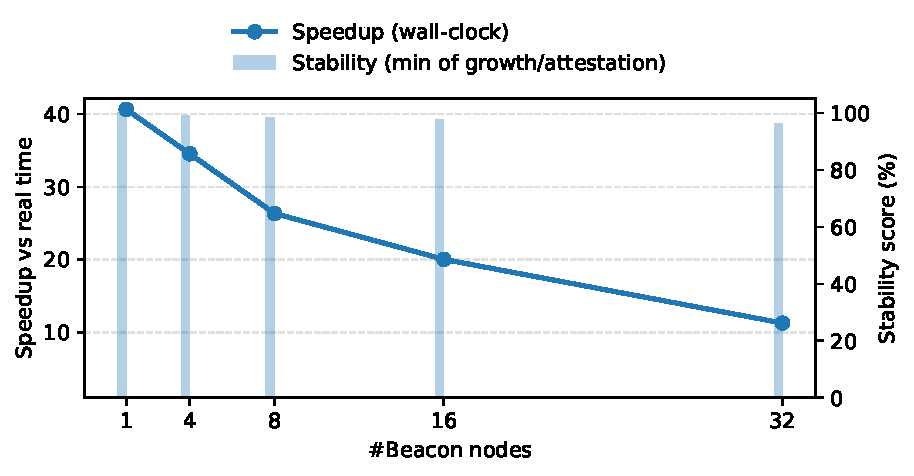
\includegraphics[width=\linewidth]{Figs/efficiency_speedup_stability.pdf}
    \caption{Speedup and stability.}
    \label{fig:efficiency_speedup_stability}
  \end{subfigure}
  \hfill
  \begin{subfigure}{0.49\textwidth}
    \centering
    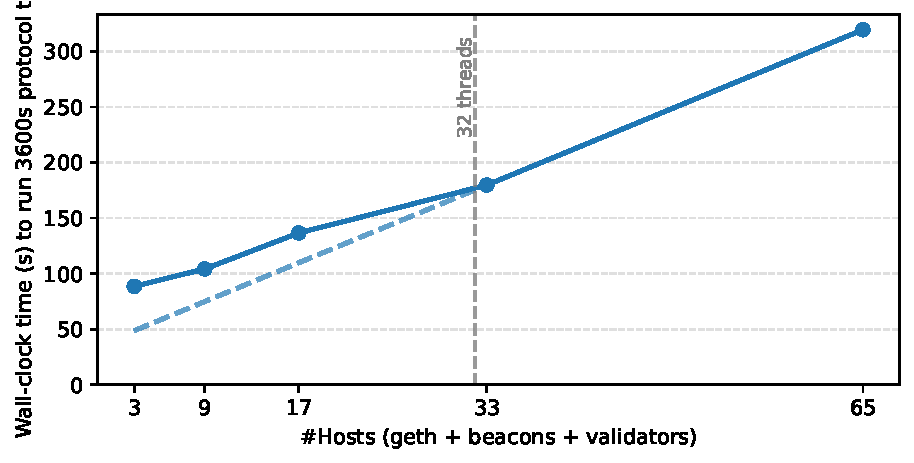
\includegraphics[width=\linewidth]{Figs/efficiency_wallclock_vs_hosts.pdf}
    \caption{Wall-clock runtime versus host count.}
    \label{fig:efficiency_wallclock_vs_hosts}
  \end{subfigure}

  \caption{Efficiency of the time-decoupled testnet on Ethereum PoS across network sizes under a fixed 3600\,s steady-state workload (300 slots). Subfigure (a) reports wall-clock speedup (line, left axis) and consensus stability (bars, right axis) for 1, 4, 8, 16, and 32 beacon-node deployments. Stability is measured as the mean attestation-inclusion percentage over epochs in the evaluation window; Growth is omitted because it remains nearly 100\% across these runs. Subfigure (b) reports wall-clock runtime of TDT for the same workload versus total simulated hosts, where $H=2B+1$ for $B$ beacon nodes in our setup (4 validators per beacon plus one shared execution layer client). The dashed guides indicate the 32-thread hardware budget and a linear reference, showing that runtime scaling becomes less favorable once the workload exceeds available hardware parallelism.}
  \label{fig:efficiency_panel}
\end{figure*}

\begin{table}[t]
\centering
\scriptsize
\setlength{\tabcolsep}{3.0pt}
\caption{Efficiency summary for the time-decoupled testnet (3600\,s steady-state workload). Speedup is $3600/T_{\mathrm{TDT}}$. Stability is the mean attestation-inclusion percentage over epochs in the evaluation window (slots 16--271) computed from beacon/validator logs; finality reports whether the run reaches the expected finalized epoch within the window (in all cases, stable $0\!\to\!6$).}
\label{tab:efficiency_speedup}
\begin{tabular}{rrrrr}
\toprule
\textbf{\#Beacons} & \textbf{Time (s)} & \textbf{Speedup} & \textbf{Att.\ incl.\ (\%)} & \textbf{Finality} \\
\midrule
1  & 88.57  & 40.7$\times$ & 100.00 & stable (0$\to$6) \\
4  & 104.23 & 34.5$\times$ & 99.20  & stable (0$\to$6) \\
8  & 136.64 & 26.3$\times$ & 98.44  & stable (0$\to$6) \\
16 & 179.74 & 20.0$\times$ & 97.85  & stable (0$\to$6) \\
32 & 319.53 & 11.3$\times$ & 96.26  & stable (0$\to$6) \\
\bottomrule
\end{tabular}
\end{table}

Figure~\ref{fig:efficiency_speedup_stability} shows that speedup decreases as network size increases, reflecting higher event volume and scheduling overhead, while consensus stability remains high across all tested sizes.
Figure~\ref{fig:efficiency_wallclock_vs_hosts} further illustrates wall-clock scaling with host count. Up to the 32-thread budget, runtime grows sublinearly, suggesting that DVN's runahead-style parallelism effectively exploits multi-core resources. Beyond this point, runtime growth becomes close to linear (e.g., the 16- to 32-beacon step nearly doubles runtime), consistent with hitting the parallelism limit and increased scheduling overhead at larger scales.

For scalability, Figure~\ref{fig:scalability_consensus_metrics} shows that RT degrades as network size increases and hits a practical bottleneck around $\sim$10 beacon nodes on the same machine: per-node Growth becomes uneven (some nodes miss most or all slots in the evaluation window), and validator voting quality degrades. Our log inspection suggests that the bottleneck is driven by deteriorating peer-communication quality under contention: as message exchange becomes less reliable, some peers accumulate lower peer scores, are disconnected, and eventually form fragmented network components, which in turn further harms consensus progress.
In contrast, TDT can stably exercise larger networks under comparable local constraints (e.g., 32 beacons in Table~\ref{tab:efficiency_speedup}). We additionally verified that a 256-beacon-node TDT deployment can still run, although at that scale substantially more wall-clock time is required to obtain one unit of logical-time progress. This reinforces the key conceptual point: once execution is decoupled from wall-clock pacing, scalability is no longer fundamentally capped by protocol time itself; in practice, it is bounded by available compute resources and event-scheduling overhead.

\begin{figure}[t]
  \centering
  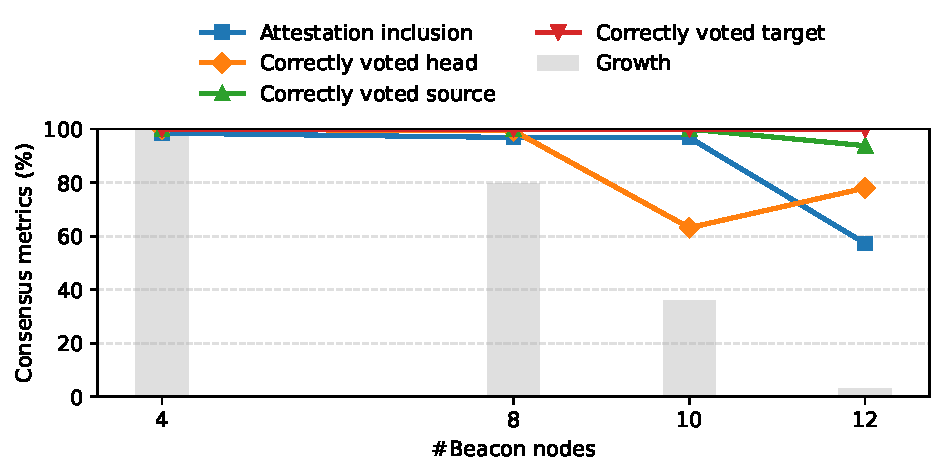
\includegraphics[width=\linewidth]{Figs/scalability_consensus_metrics.pdf}
  \caption{Consensus metrics of the real-time testnet (RT) as network size increases over the 256-slot evaluation window (slots 16--271). Growth is the per-node block synchronization rate extracted from beacon logs. The validator curves are derived from each node's \texttt{Vote summary since launch} lines, including attestation-inclusion percentage and correctly-voted head/source/target percentages. All metrics are shown on a 0--100\% scale (Growth scaled by 100) and averaged across nodes with available summaries. The figure highlights the degradation of consensus quality as RT approaches its local deployment limit.}
  \label{fig:scalability_consensus_metrics}
\end{figure}

\smallskip
\noindent\textbf{Takeaway.}
In direct answer to \textbf{Q2}, TDT substantially reduces wall-clock time for a fixed logical-time workload, delivering order-of-magnitude speedups across 1--32 beacon nodes while maintaining robust consensus advancement. At the same time, under a fixed local machine budget, RT encounters a practical scalability bottleneck around $\sim$10 beacon nodes (Figure~\ref{fig:scalability_consensus_metrics}), whereas TDT continues to exercise substantially larger networks; we additionally verified that a 256-beacon-node TDT deployment can still run, albeit with much higher wall-clock cost per unit of logical time. This result highlights the main benefit of removing the wall-clock \emph{time lock}: the practical limit shifts away from protocol-time pacing and toward ordinary system constraints such as available compute and event-scheduling overhead, rather than an inherent real-time bound on protocol progress.


\subsection{Testing Effectiveness: Exercising the Consensus State Machine}
\label{subsec:eval_effectiveness}

This subsection answers \textbf{Q3}: \emph{Under a fixed wall-clock testing budget, how much more of the consensus state machine can we exercise?} Our core claim is that the dominant bottleneck in PoS testnet testing is the \emph{time lock}, which limits how densely the consensus state machine can be exercised under conventional wall-clock execution.

We therefore measure testing effectiveness in terms of \emph{consensus core-logic execution density per unit wall-clock budget}. Our setup mirrors Section~\ref{subsec:sparsity}: 8 beacon nodes with 16 validators, sharing one Geth execution client. Using the instrumented \texttt{spec.log} traces, we compute per-category invocation densities on a representative node. Calls per protocol second characterize the logical workload itself, while calls per wall-clock second characterize the practical testing throughput observed by the experimenter.

\begin{table}[t]
\centering
\scriptsize
\setlength{\tabcolsep}{3.5pt}
\caption{Core-logic invocation density for the 8-node time-decoupled testnet setup (node-2), extracted from instrumented \texttt{spec.log} traces. Calls per protocol second measure the logical workload, calls per wall-clock second measure practical testing throughput, and the density gain reports how much more state-machine work TDT fits into the same wall-clock budget.}
\label{tab:effectiveness_corelogic_density_edt8}
\begin{tabular}{lrr}
\toprule
\textbf{Category} & \textbf{Calls / protocol s} & \textbf{Calls / wall s} \\
\midrule
Total      & 14.15 & 358.17 \\
Block      & 9.45  & 239.33 \\
Epoch      & 1.64  & 41.47 \\
Forkchoice & 1.32  & 33.49 \\
State      & 1.32  & 33.44 \\
Validator  & 0.41  & 10.45 \\
\bottomrule
\end{tabular}
\end{table}

Table~\ref{tab:effectiveness_corelogic_density_edt8} directly answers Q3. On the representative node, total core-logic execution density rises from 14.15 calls per protocol second to 358.17 calls per wall-clock second, corresponding to a 25.3$\times$ density gain. Similar gains appear across all major categories---block processing, epoch processing, fork choice, state transitions, and validator duties---showing that TDT does not merely accelerate one hot path. Instead, by unlocking the \emph{time lock}, it converts long protocol waiting intervals into useful state-machine exercise across the full consensus workflow.

This higher iteration rate is also \emph{controllable}: testers can deterministically choose time windows and schedules, enabling repeatable experiments and targeted stress cases rather than merely obtaining a faster but opaque execution.

To make the density gain tangible, Figure~\ref{fig:corelogic_density_edt8_wallclock60s} visualizes per-category core-logic invocation rates within a fixed 60\,s wall-clock window on TDT. In a conventional wall-clock testnet, most of this budget would be spent waiting for the next slot or epoch boundary. In TDT, the same wall-clock budget is converted into sustained, repeated execution of time-triggered and message-triggered consensus logic.

\begin{figure}[t]
  \centering
  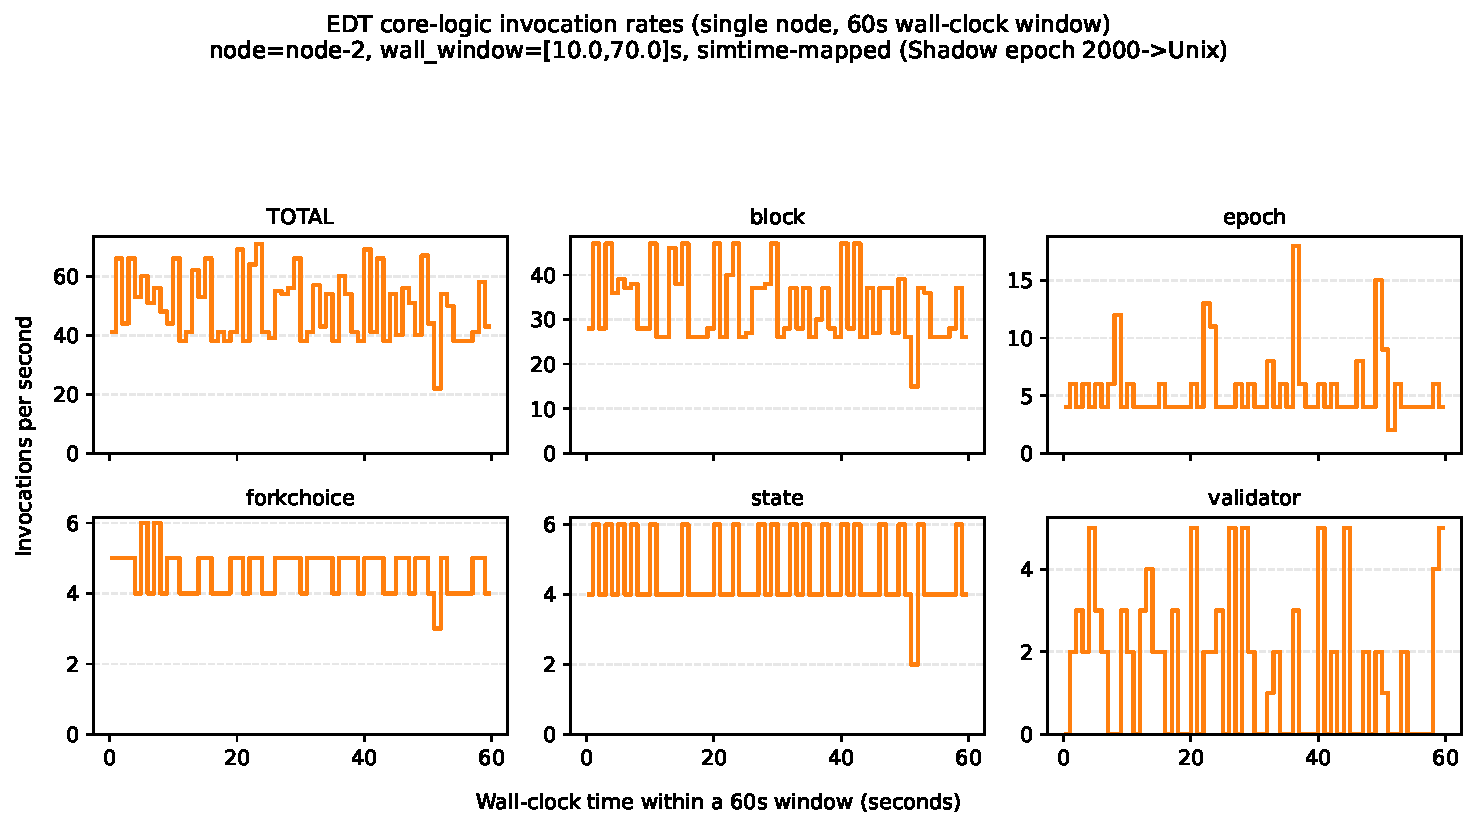
\includegraphics[width=\linewidth]{Figs/corelogic_density_edt8_wallclock60s_2x3.pdf}
  \caption{Core-logic invocation rates in the 8-node time-decoupled testnet over a fixed 60\,s wall-clock window, using 3\,s buckets. The six subplots report \textsc{Total}/block/epoch/forkchoice/state/validator call rates (calls per second) within the same window, showing how TDT compresses protocol waiting time into dense, observable state-machine execution.}
  \label{fig:corelogic_density_edt8_wallclock60s}
\end{figure}

\smallskip
\noindent\textbf{Takeaway.}
In direct answer to \textbf{Q3}, TDT allows substantially more of the consensus state machine to be exercised within the same wall-clock budget. This is a central contribution of the framework: not just faster execution, but a qualitatively more effective testing regime for strongly time-controlled protocols. It enables higher-throughput stateful fuzzing (higher feedback rate for time-triggered logic), faster regression testing across many epochs, systematic exploration of fault schedules for chaos testing, and reproducible debugging via re-running the same time-windowed execution under fixed seeds and schedules.

\subsection{Operational Utility}
\label{subsec:eval_case_debug}

This subsection answers \textbf{Q4}: \emph{Can the framework support a practical replay-and-debug workflow for timing-sensitive consensus events, rather than merely accelerating execution?} We answer this question in two parts. First, we show that TDT supports reproducible debugging of a shallow reorg by returning to the same logical-time window and inspecting real client processes around the event. Second, we show that TDT can host an existing message-driven fuzzer, \textsc{LOKI}, clarifying both what TDT already enables and what remains outside the reach of a purely message-driven strategy.

\smallskip
\noindent\textbf{Case Study: Debugging a shallow reorg.}
We evaluate this workflow on the same Prysm+Geth deployment used in the fidelity study: 4 beacon nodes, 16 validators, and one shared execution client, running under the DVN latency model with mean 100\,ms and a fixed random seed. Under this intentionally noisy but deterministic setting, a shallow reorg is repeatedly triggered within the same logical-time window, as discussed in Section~\ref{subsec:eval_fidelity}.

The operational benefit is that the event can be revisited as a \emph{debug target} rather than merely observed once.
First, we run a 30-minute testnet execution in TDT and observe several shallow reorgs, as expected under the intentionally noisy latency model.
We then inspect the client logs to locate a target reorg window. For clarity, Table~\ref{tab:reorg_window_timeline} summarizes the key events observed on node-1.

\begin{table}[t]
\centering
\scriptsize
\setlength{\tabcolsep}{4pt}
\caption{Key events in the target shallow-reorg window observed. For ease of presentation, we refer to the block at slot $s$ as \emph{block $s$}.}
\label{tab:reorg_window_timeline}
\begin{tabular}{p{0.16\linewidth}p{0.22\linewidth}p{0.52\linewidth}}
\toprule
\textbf{Time} & \textbf{Event} & \textbf{Key observation} \\
\midrule
14:05:47 & Sync block 63 & Node-1 syncs \emph{block 63} (\texttt{0x3044efb7...}), which later appears as the common ancestor of the reorg. \\
14:06:02 & Sync block 64 & Node-1 accepts \emph{block 64} (\texttt{0xcdb4b141...}) as the current chain continuation. \\
14:06:10 & Reorg warning & The client reports a reorg from old root \texttt{0xcdb4b141...} (slot 64) to new root \texttt{0xea3f3027...} (slot 65), with common ancestor \texttt{0x3044efb7...}. \\
14:06:10 & Sync block 65 & Node-1 switches to the competing branch and syncs \emph{block 65} (\texttt{0xea3f3027...}) as the new canonical head. \\
\bottomrule
\end{tabular}
\end{table}

We can see that this log shows that the fork diverges after the block at slot 63, which we denote as \emph{block 63}, with root \texttt{0x3044efb7...}; this block is later reported as the common ancestor of the reorg. The node first accepts the block at slot 64, denoted as \emph{block 64}, with root \texttt{0xcdb4b141...} as the current continuation of the chain. A few seconds later, however, the client reports a chain reorg and switches to a competing branch whose new canonical head is the block at slot 65, denoted as \emph{block 65}, with root \texttt{0xea3f3027...}.

In other words, the history after block 63 temporarily contains two conflicting versions of ``what happened next'': one branch in which block 64 is treated as the head, and another branch that supersedes it and advances to block 65. From a debugging perspective, this is exactly the kind of timing-sensitive episode we want to revisit: the experimenter can focus on the narrow logical-time window around blocks 63--65 and inspect why the node first followed one post-fork branch and then switched to another.

Starting from the same configuration and seed, the experimenter can replay the run, return to the same logical-time interval, and pause at a safe boundary before the reorg window around blocks 63--65. Concretely, we pause at slot 63 and inspect the proposer and voting behavior in the following two slots.

The replay shows that node-2 is selected as the proposer for block 63, and this block is already late: block's construction finishes at \texttt{sinceSlotStartTime=2.9s}, whereas in normal slots we typically observe roughly 1.3--1.5\,s. As a result, when the voting period for slot 63 begins, only node-1 and node-2 have already observed block 63, while node-3 and node-4 are still voting on the previous head. Even so, block 63 still receives enough support to remain the canonical base for the next slot.

The more important step is what happens next. Because the network is small, the probability that the same node is selected to propose again in the next slot is relatively high; in this run, node-2 also proposes block 64. However, block 64 is built even later, with \texttt{sinceSlotStartTime=5.1s}. By the time it is disseminated, the voting period for slot 64 has effectively passed, so validators can only attest to block 63 rather than to block 64. In other words, block 64 is a valid extension of block 63, but it is a \emph{late block} that fails to gather timely attestation support.

Under these conditions, a shallow reorg is not surprising. Once another branch advances and obtains the weight that block 64 failed to accumulate, the fork choice naturally abandons block 64 and switches to the branch headed by block 65. The key point of this case study is therefore not that the reorg reveals a protocol bug, but that TDT lets us deterministically reconstruct \emph{why} the reorg happened: a small network, consecutive proposer selection on node-2, and transient network delay together produced a late block with insufficient votes, making reorg replacement entirely normal.

This turns a transient timing-sensitive event into a repeatable debugging workflow. Instead of treating the reorg as an opaque one-off outcome, the experimenter can pause before the critical window, inspect the corresponding real client processes, logs, proposer timing, and peer observations, and then reason about how alternative fault schedules or message timings would have changed the same consensus episode. 

The present example is only a shallow and ultimately explainable reorg; the value of this workflow becomes even greater for more complex events, especially when the root cause may involve subtle implementation or code-level issues rather than an expected consequence of timing and network variation alone.


\smallskip
\noindent\textbf{Message-Driven Fuzzing Compatibility.}
We also run a migrated version of \textsc{LOKI}~\cite{ma2023loki} inside TDT to evaluate whether the framework can support existing message-driven fuzzing workflows. In practice, this adaptation requires almost no structural modification to the fuzzer itself: we keep \textsc{LOKI}'s original mutation logic, message-oriented testing strategy, and harness structure, and only adjust the distribution of message injection so that it better matches the more rapidly changing consensus state machine under TDT. This shows that TDT is directly compatible with existing network-level fuzzers and can provide them with faster, more controllable executions without requiring a redesign from scratch.

Deterministic replay provides an additional operational advantage for fuzzing. Once a bug-triggering execution is found, the same seed and configuration can be replayed inside TDT so that the failure can be re-observed and debugged precisely, rather than being treated as a one-off fuzzing artifact. This matters because, in conventional distributed testnets, failures are often difficult to trace after the fact: even when an important error is observed, it may be impossible to reproduce it reliably or to localize its root cause, simply because the full distributed state of the testnet is hard to preserve at low cost. This is a common challenge in distributed fuzzing and large-scale system testing more broadly. By making the execution schedule reproducible, TDT turns a transient failure from an ephemeral observation into a stable debugging target. In this sense, TDT improves not only the speed of campaign execution, but also the post-discovery analysis workflow.

\smallskip
\noindent\textbf{Limitations and Future.}
At the same time, our experience clarifies two current limitations. First, fuzzing often requires long campaigns before a bug is discovered. If a failure is only found after, for example, ten hours of execution, then replaying that failure currently also requires replaying roughly the same ten-hour prefix. A more lightweight replay mechanism that can jump directly to the target logical-time region remains future work.

Second, the bugs exposed by the current \textsc{LOKI}-style setup are still predominantly p2p-layer implementation bugs rather than time-gated consensus-core bugs. This is expected: a message-driven fuzzer mainly perturbs message handling, peer management, discovery, sync, and other network-facing code paths, and it does not collect consensus-level feedback to guide mutation toward slot/epoch-triggered logic. 

Historically, this design choice is also understandable: under conventional real-time testnets, the consensus state machine advances too slowly and too sparsely for consensus-level feedback to be collected at a useful rate, so earlier fuzzers effectively gave up on using such feedback at all. TDT changes this premise. By making consensus-state progression much denser under the same wall-clock budget, it makes automated fuzzing against consensus core logic practically attainable rather than prohibitively expensive. In other words, TDT makes message-driven fuzzing faster and more replayable, and it also creates the conditions for a stronger next step: a new fuzzer designed specifically for TDT---one that uses consensus-aware or timing-aware feedback to guide mutation---is therefore a natural and promising direction for future work.

\smallskip
\noindent\textbf{Bug disclosure.}
During TDT-integrated fuzzing experiments, after three campaign runs of roughly 10 hours each, we encountered four p2p-layer implementation bugs and reported them to the client communities. One has already been fixed in a subsequent release, while the other three remain under discussion at the time of writing.

Although these findings are modest, they illustrate an important practical point: running real, unmodified clients inside a controllable testnet can indeed expose implementation bugs, rather than merely protocol-level phenomena. In this sense, TDT retains the fundamental advantage of testnet-based evaluation over simulation: unlike a simulator, it exercises the actual deployed code paths and can therefore reveal real implementation defects while still providing reproducibility and control.

\smallskip
\noindent\textbf{Takeaway.}
In direct answer to \textbf{Q4}, TDT provides practical operational utility beyond raw acceleration. It turns transient timing-sensitive events into replayable debugging targets, supports existing message-driven fuzzers such as \textsc{LOKI} with almost no structural modification, and enables precise post-failure analysis through deterministic replay. Our TDT-integrated fuzzing campaigns also surfaced real p2p-layer implementation bugs in unmodified clients, highlighting that the framework retains the key advantage of testnet-based evaluation over simulation: it can expose actual implementation defects while remaining controllable and reproducible. At the same time, our experience shows that moving bug discovery from the p2p surface into consensus core logic will require a new generation of timing-aware fuzzers built specifically to exploit the denser consensus feedback that TDT makes available.

\section{Related Works}

\section{Conclusion}\label{sec:conclusion}

This paper argues that the central limitation of conventional testnets for strongly time-controlled consensus is not merely that they are ``slow,'' but that they are \emph{time-locked}: protocol time remains bound to wall-clock execution, so a large fraction of testing effort is spent waiting rather than exercising the consensus state machine. To address this limitation, we presented a time-decoupled testnet (TDT), a methodology that decouples logical protocol time from wall-clock execution while still running real, unmodified client binaries end to end.

Our design preserves protocol-time semantics and implementation fidelity while making execution controllable and reproducible. On Ethereum PoS, our evaluation shows that TDT preserves the key consensus behaviors of interest, delivers order-of-magnitude wall-clock speedups, increases consensus core-logic execution density by roughly 25$\times$ under the same wall-clock budget, and supports practical replay-and-debug workflows for timing-sensitive events. The operational case studies further show that TDT can host existing message-driven fuzzers with minimal adaptation, enables precise replay of discovered failures, and can surface real implementation bugs in deployed clients---retaining the fundamental advantage of testnet-based evaluation over simulation while overcoming the time-lock bottleneck.

More broadly, we view TDT as an enabling foundation for security evaluation of time-critical consensus protocols. By turning logical-time windows into controllable, replayable units of execution, it makes faster attack replay, denser automated testing, and reproducible debugging substantially more practical. Future work includes lighter-weight replay mechanisms, broader client and protocol support, and, most importantly, a new generation of timing-aware fuzzers that can exploit the denser consensus feedback that TDT makes possible.

